\subsection{Scenario 1 - Homework submission}

Alice wants to submit a homework for her Python course. She has already finished it and written some code in 2 files, named ``IO\_Input.py'' and ``IO\_Output.py''.

She logs onto jGrader and sees homework 5 on the landing page. She clicks a button and is brought to the submission page. Alice clicks on the slot and selects the file from her computer. A progress bar appears while the file is being uploaded.

She opens the jGrader homepage and sees that it is due very soon, this week

On the same page a ``Upload files'' field appears.

Alice finds the file on her computer and drags it into the field that just appeared. Because the file is very big (it contains a lot of scanned images) jGrader shows a progress bar while the file is uploaded. After a few seconds, the upload finishes and Alice gets a confirmation that the file was indeed uploaded. She then close the page.


Alice is taking Python this year which she uses our grading platform for. When she is is on the student landing page.\\

\includegraphics[width=\textwidth]{screenshots/StudentLandingPage.png}\\

From there she realizes that the next assignment due is for Python Lab. Alice clicks on the \textit{Current courses} to have an overview of all her courses.\\
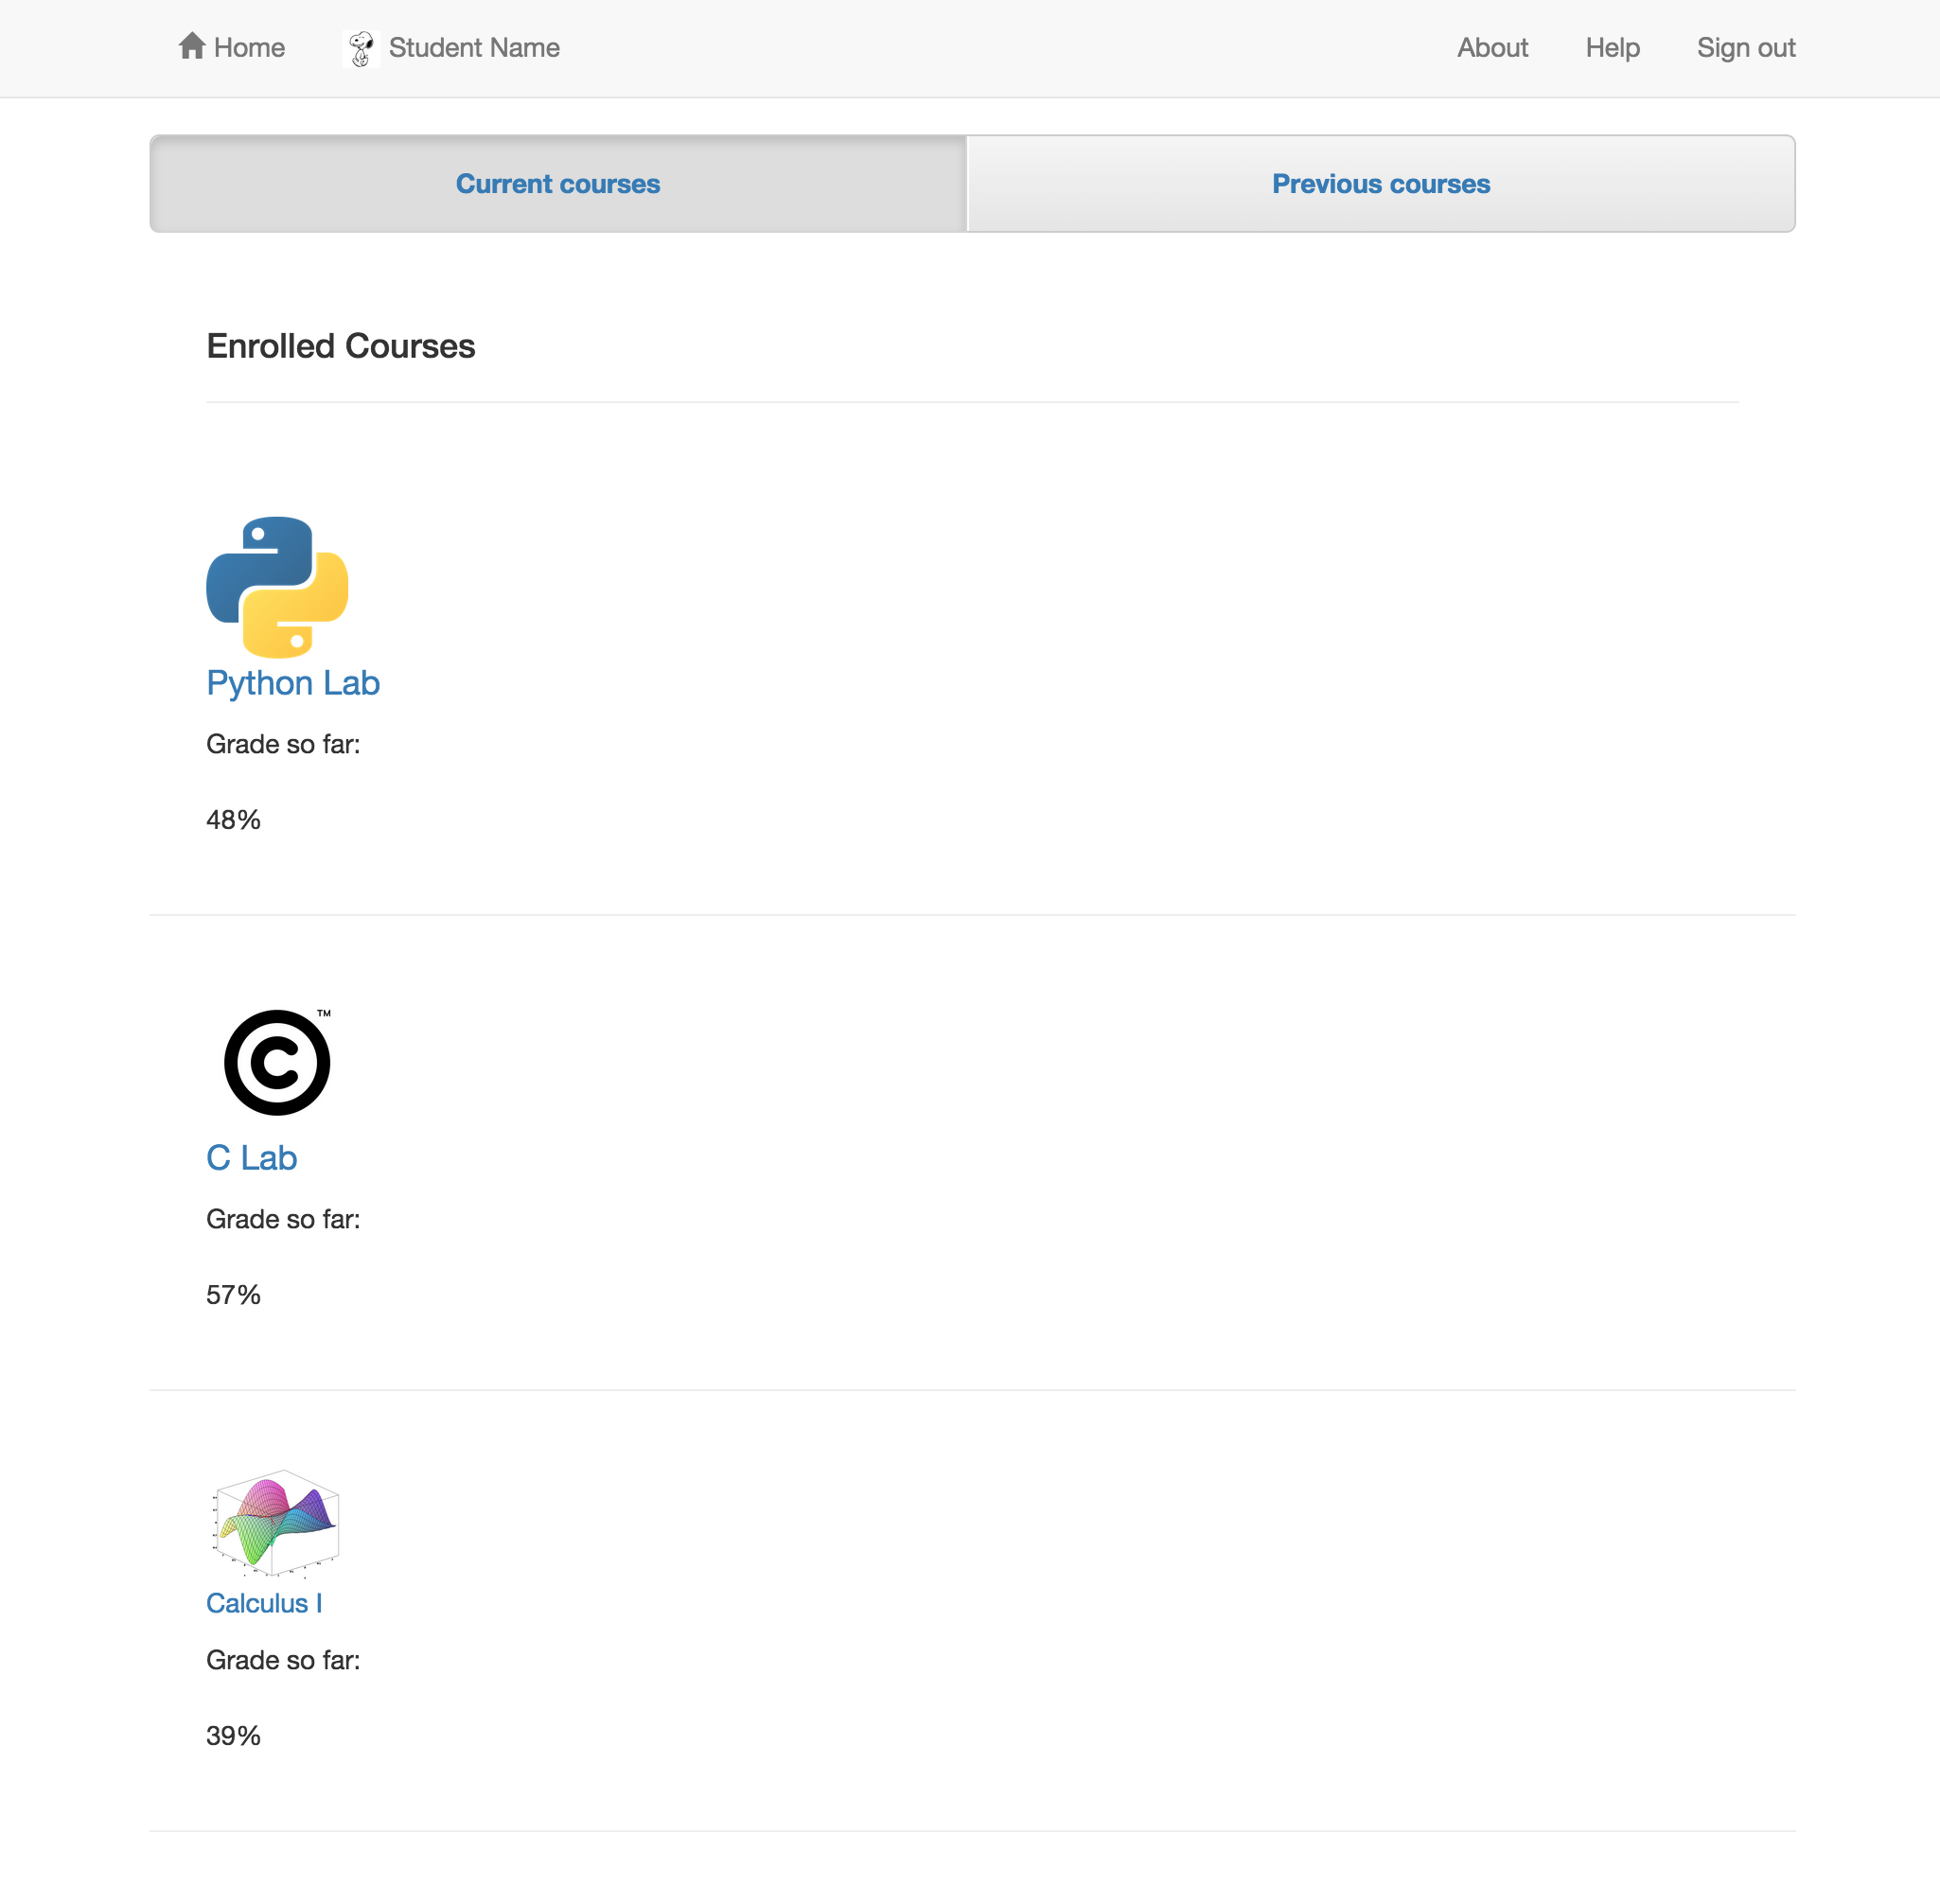
\includegraphics[width=\textwidth]{screenshots/CurrentCourses}\\
Since she still has to do her Python homework assignment she navigates to the Python Lab.\\
The course page layout is designed to provide an easy to use and comprehensive dashboard for each course. It contains current assignments, previous assignments, tools to view further information, request extensions \& excuses, and an overview of the course grading breakdown, instructors, credits, and other important information.\\

On the top of the page Alice can choose the current homework screen or the previous homework Assignments screen. On the current homework screen the most frequently accessed elements are at the top of the screen to minimize scrolling and allow for easy accessibility. Hence the first information is when the deadline for the current assignment it and right below it is a huge submit button that cannot be missed. Apart from this it also has buttons to view the current assignment, to request and extension, and to request an excuse. The colors for the buttons are green, yellow, and red respectively which underlines how crucial the respective action is. E.g. requesting an excuse is a more crucial action than requesting an extension.\\

Below the buttons that allow Alice to perform actions, the course page offers information about the course and the grading criteria. Being naturally curious about the grades she received on previous homework assignments, she goes to that section and can see her previous submissions and the grades she received for them in a nicely formatted table.\\
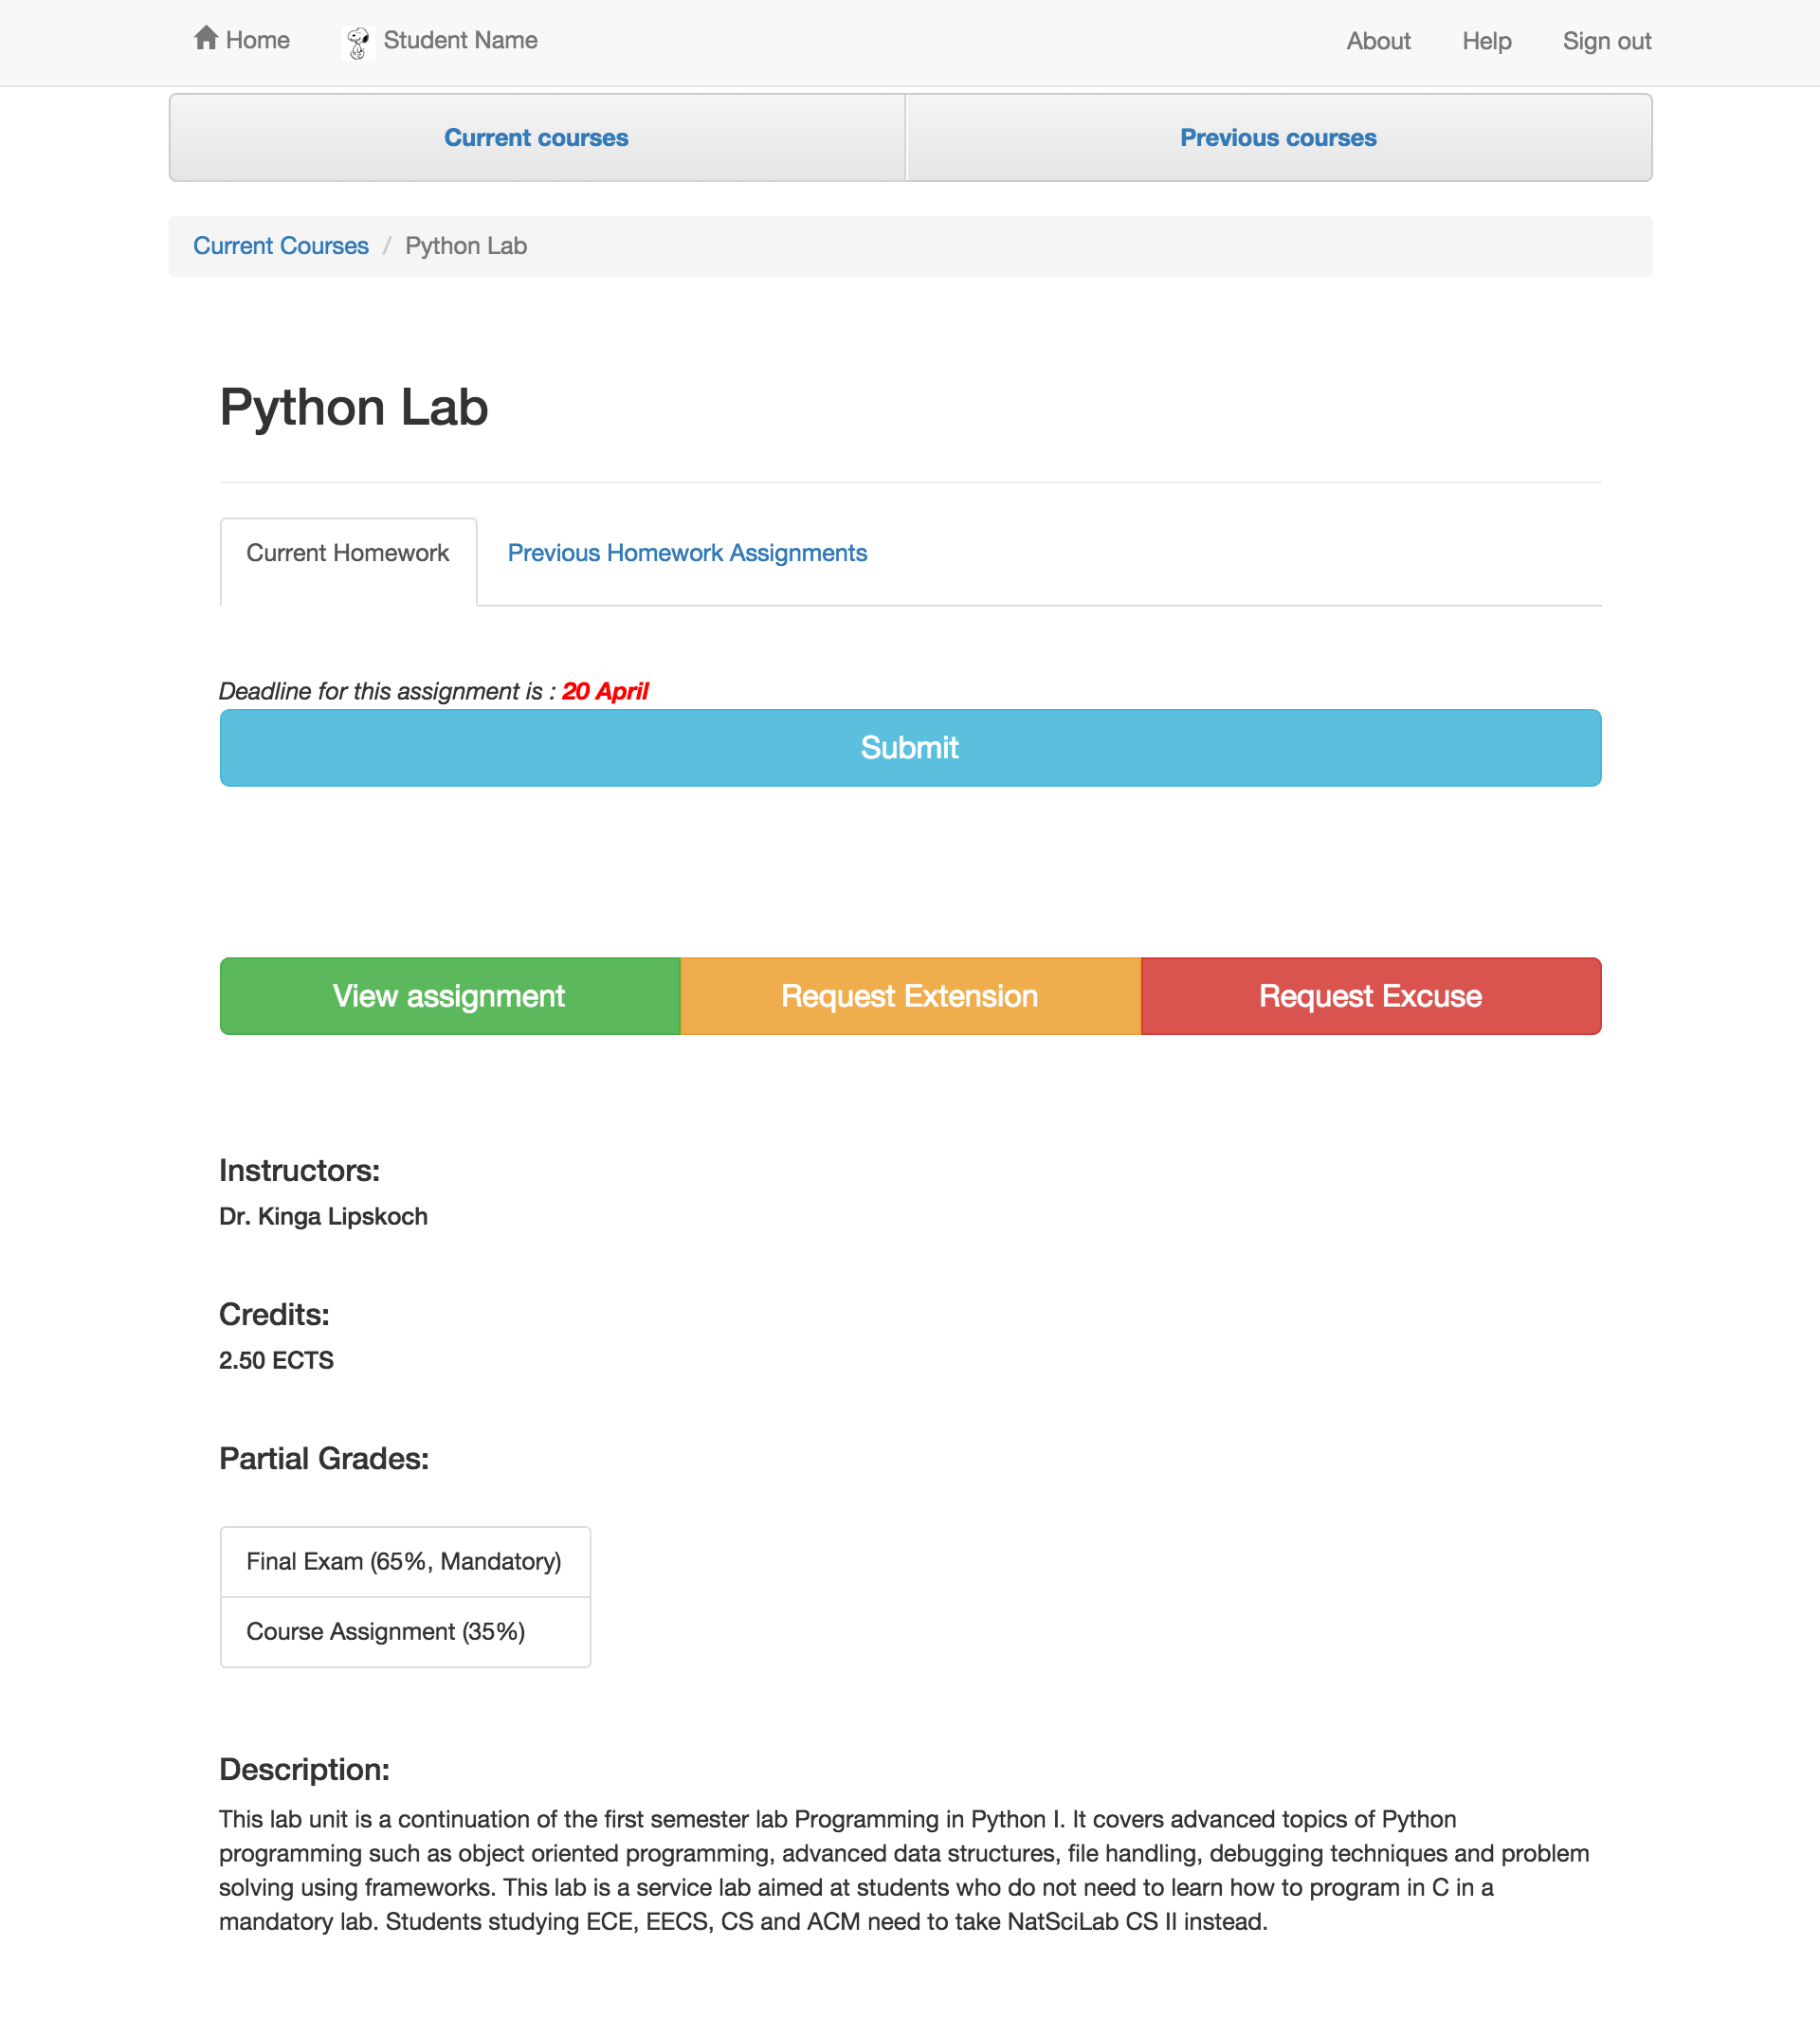
\includegraphics[width=\textwidth]{screenshots/PreviousHW}\\

Going back to the current homework page, Alice wants to now submit her current homework assignment. For that she clicks on the submit button and is redirected to the submission page.\\
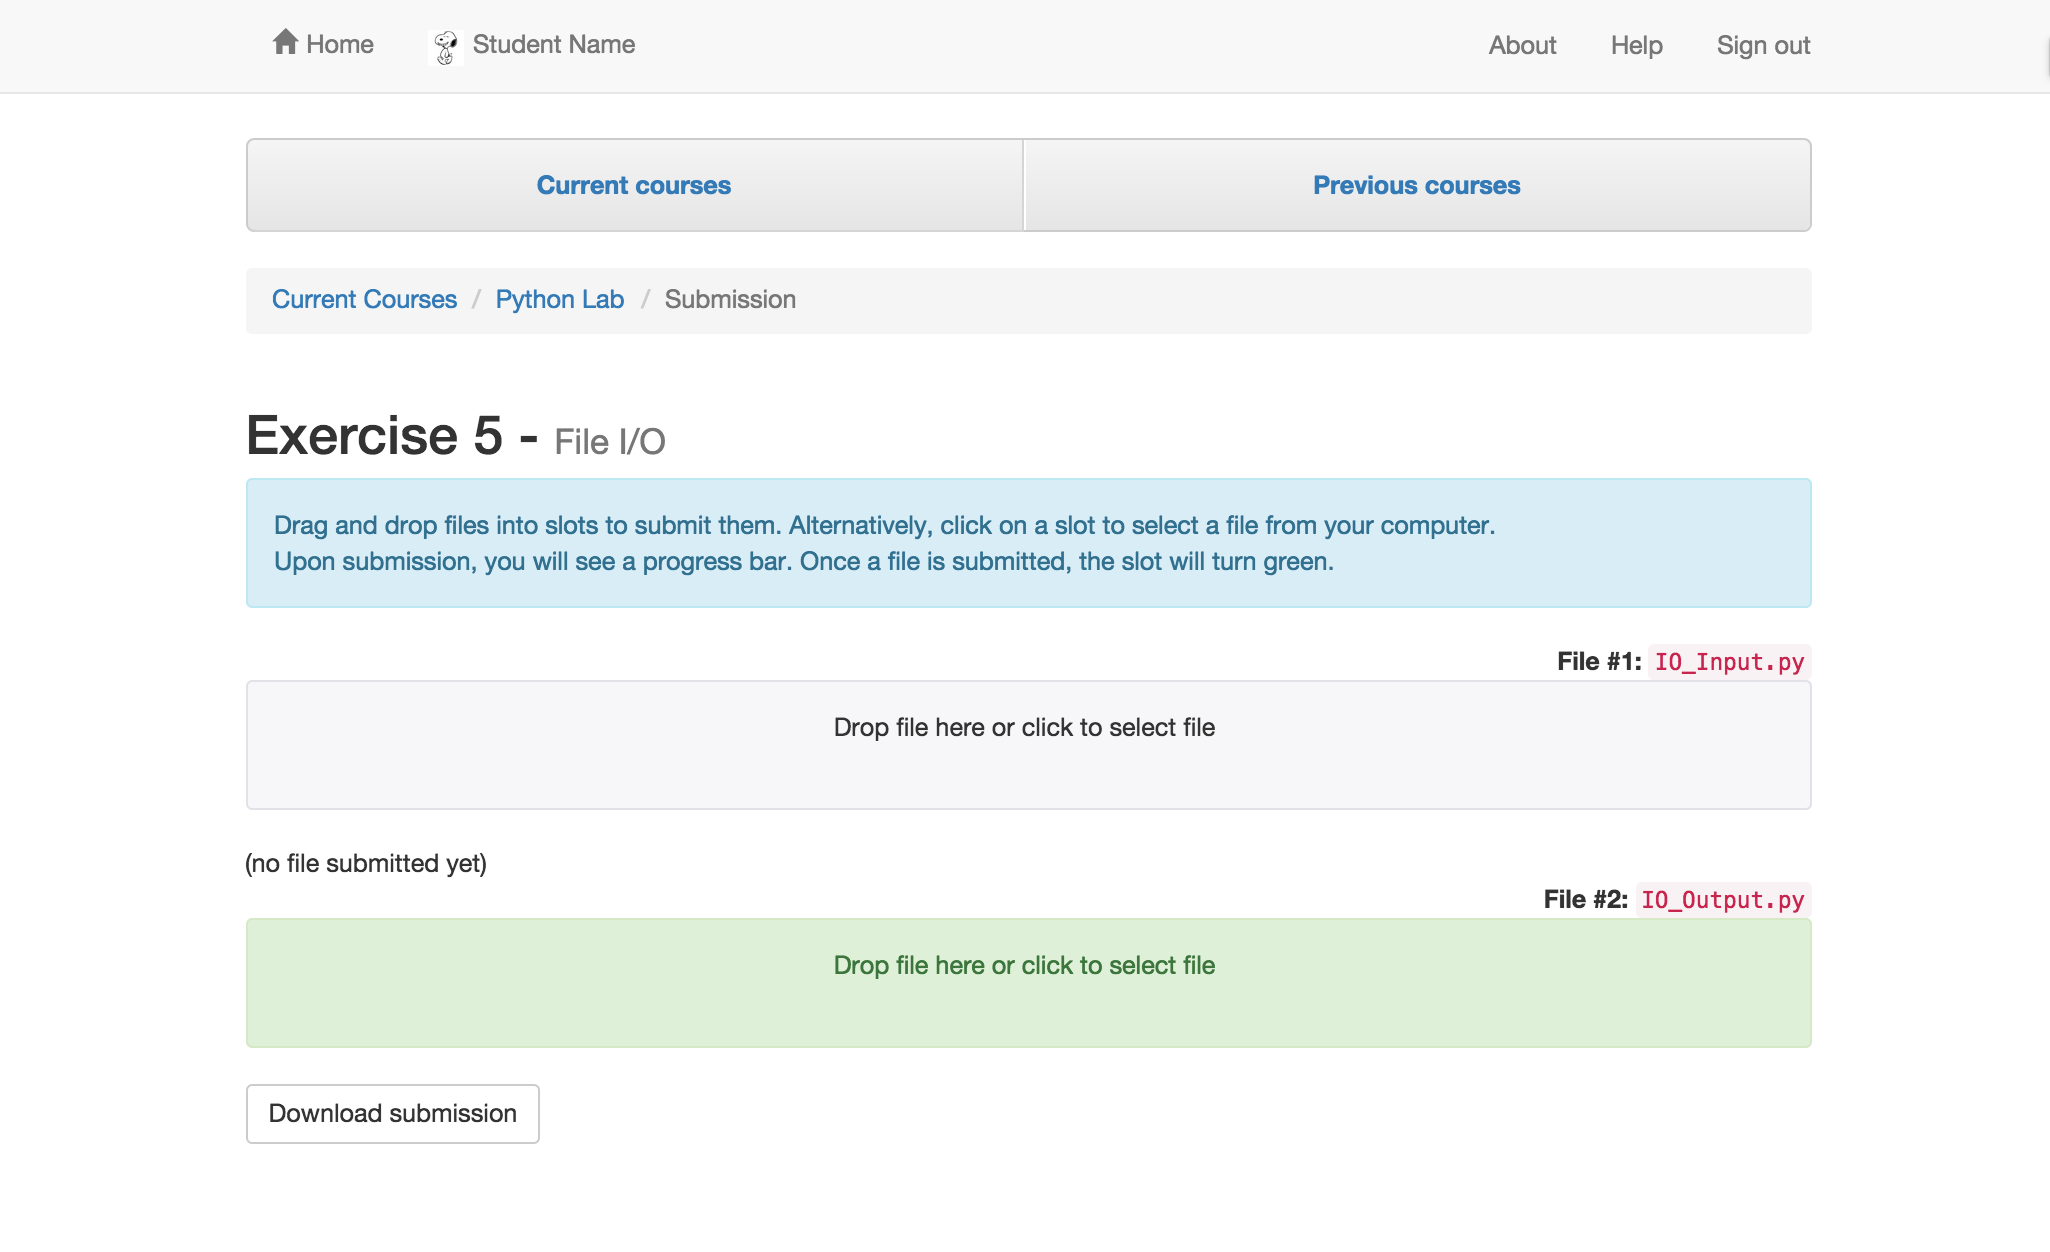
\includegraphics[width=\textwidth]{screenshots/Exercise5}
